\chapter{Theoretical Background}
\label{cha:theory}

\section{Statistical thermodynamics and free energy differences}
\label{sec:freeE}

The formulation of the problem of free energy estimation starts with the Hamiltonian
\begin{equation}
  \textbf{H}(\textbf{x},\textbf{p})=\sum_{i=0}^{N}\frac{p_{i}^{ 2}}{2 m_i} + U(\textbf{x})
\end{equation}
of an arbitrary chemical system, where $(\textbf{x},\textbf{p})$ denotes a point in the phase space of the N-particle system of interest with atomic coordinates $\textbf{x}=(x_1, ..., x_N)$, momenta $\textbf{p}=(p_1,...,p_N)$ and masses $(m_1,...,m_N)$. $U(\textbf{x})$ is the potential energy given by any quantum chemical method or force field. If the canonical (N,V,T)-ensemble of such a system is sampled, for example by means of Langevin dynamics or Monte Carlo simulations, the probability distribution $\rho(\textbf{x})$ in the configuration space $\textbf{x}$ follows the Boltzmann distribution
\begin{equation}
  \rho(\textbf{x})=\frac{e^{-\beta U(\textbf{x})}}{\int e^{-\beta U(\textbf{x})} d\textbf{x}}=Z^{-1}e^{-\beta U(\textbf{x})}
  \label{eq:boltzmann}
\end{equation}
were $Z$ denotes the partition function and $\beta=(k_B T)^{-1}$ the inverse temperature with Boltzmann constant $k_B$.
%By acting as normalization constant to ensure $\int\rho(x)dx=1$, the partition function is the central quantity of statistical thermodynamics, relating macroscopic thermodynamic quantities to the microscopic details of a system.
In this work we will focus on alchemical transformations, $A\longrightarrow B$, which are represented by a small set of collective variables (CV's) $(\xi_1(\textbf{x}) : \mathbb{R} ^{3N} \to \mathbb{R}, ..., \xi_n(\textbf{x}))$, that are sufficient to distinguish between key states of interest.
In this framework the probability distribution can be expressed by a histogram along collective variables
\begin{equation}
  \rho(\xi)=\int \delta[\xi-\xi(\textbf{x})]\rho(\textbf{x})=\braket{\delta [\xi -\xi(\textbf{x})]}_\xi
  \label{eq:rho}
\end{equation}
where $\braket{}_\xi$ denotes the $\xi$-conditioned marginal distribution and the free energy difference between two states A and B is defined as
\begin{equation}
  \Delta A_{A\rightarrow B} = -\beta^{-1}\ln \frac{\rho(\xi(\textbf{x}_B))}{\rho(\xi(\textbf{x}_A))}
  \label{eq:free energy unbiased}
\end{equation}
However, in computer simulations the direct phase-space integrals used in equation  \ref{eq:boltzmann} and \ref{eq:rho} are impossible to calculate. Instead the time average $P(\xi)$ is computed by monitoring $\xi$ during the simulation.
\begin{equation}
  P(\xi)=\lim_{t\rightarrow \infty}\frac{1}{t} \int_0^t \rho[\xi (t')] dt'
  \label{eq:ergodic}
\end{equation}
In practice, $P(\xi)$ is approximated as a histogram along the reaction coordinate with bins of fixed size.
Assuming that the system at hand behaves \textit{ergodic}, i.e. every point in phase space is visited during a infinitely long simulation, the ensemble average $\rho(\xi)$ converges to the time average $P(\xi)$ for long simulations. However, transitions of high energy barriers during chemical reactions are typically rare events, that might happen on timescales far beyond what is feasible to compute. Therefore most processes, for example in biochemical context, are \textit{quasinonergodic}. The problem of calculating accurate free energy differences hence really consists in adequate sampling of regions with high free energy (transition states) along the reaction coordinate.

For this purpose several \textit{enhanced sampling} methods were developed.\autocite{} In this work we will focus on CV-based approaches, that are based on altering the potential energy in a way, that increases the time spent in a certain region of configuration space during a simulation. One of the oldest and simplest methods to achieve the same is \textit{Umbrella Sampling} (US). In its most common form US introduces an fixed harmonic bias potentials of the form
\begin{equation}
  U_{B}(\xi) = \frac{k_i}{2}(\xi(t)-\xi_i)^2
\end{equation}
where the index i indicates a given bias window along the reaction coordinate with force constant $k_i$.

<reweighting and WHAM>

\section{Adaptive Biasing Methods}
\label{sec:adaptive biasing}

Instead of dividing the reaction coordinate in several windows, with adaptive biasing methods the free energy can be estimated from one single simulation. For this purpose the systems dynamics are biased towards states corresponding to large values of the free energy along the transition coordinate via a history-dependent biasing potential. In contrast to other importance sampling strategies like umbrella sampling, this methods require no prior knowledge of the free-energy landscape at hand. Instead, the biasing potential automatically converges towards the free energy, enabling diffusive behavior along the transition coordinate.

There are multiple adaptive biasing methods available, only differing in the construction of the bias. Methods based on metadynamics (metaD) disfavor already visited states by accumulating repulsive potentials along the CV (section \ref{sec:metaD}), while adaptive biasing force (ABF) methods compensate the mean force along the reaction coordinate to obtain uniform sampling (section \ref{sec:ABF}). Meta-eABF finally combines both complementary approaches to further speed up convergence (section \ref{sec:meta-eABF}).

In principle adaptive biasing methods only rely on the sampling of the canonical ensemble, which will be obtained using Langevin dynamics in this work. A schematic procedure of adaptively biased Langevin dynamics is given in Algorithm \ref{alg:ABM}.

\begin{algorithm}[H]
  \caption{Velocity Verlet integrator for adaptively biased Langevin dynamics with atomic masses $\textbf{M}$, coordinates $\textbf{x}(t)$, momenta $\textbf{p}(t)$, potential $V(\textbf{x}(t))$, forces $F(\textbf{x}(t))$ and friction coefficient $\gamma$,}
  \label{alg:ABM}
    \begin{algorithmic}
      \WHILE{$t < t_{end}$}
        \STATE
        \STATE $\textbf{p}(t+\frac{1}{2}\Delta t) \leftarrow \textbf{p}(t) + \frac{1}{2} \bigl(F(\textbf{x}(t))dt-\gamma \textbf{M}^{-1}\textbf{p}(t) dt + \sqrt{2\gamma\beta^{-1}}dW_t \bigr)$
        \STATE $\textbf{x}(t+\Delta t) \leftarrow \textbf{x}(t) + \frac{2}{2+\gamma dt}\textbf{M}^{-1} \textbf{p}(t+\frac{1}{2}\Delta t) dt$
        \STATE /* Langevin dynamics
        \STATE
        \STATE $F(\textbf{x}(t+\Delta t)) \leftarrow -\nabla U(\textbf{x}(t+\Delta t))$
        \STATE /* get physical QM/MM forces
        \STATE
        \STATE $\xi \leftarrow f(\textbf{x}(t+\Delta t))$
        \STATE /* Calculate reaction coordinate from Cartesian coordinates
        \STATE
        \IF{$\xi_{min}\leq\xi\leq\xi_{max}$}
          \STATE
          \STATE $F_{B}(\xi, t+\Delta t))\leftarrow F_{B}(\xi, t))+\Delta F_{B}(\xi,t+\Delta t))$
          \STATE /* update history dependent bias force along reaction coordinate incrementally
          \STATE
          \STATE $F(\textbf{x}(t+\Delta t)) \leftarrow -\nabla U(\textbf{x}(t+\Delta t)) + F_{B}(\xi, t+\Delta t))\nabla\xi$
          \STATE /* Add biasing force to physical force
          \STATE
        \ELSE
          \STATE
          \STATE $F(\textbf{x}(t+\Delta t)) \leftarrow -\nabla U(\textbf{x}(t+\Delta t)) + k\min(|\xi-\xi_{min}|,|\xi-\xi_{max}|)\nabla\xi$
          \STATE /* confine to range of interest with force constant $k$
          \STATE
        \ENDIF
        \STATE
        \STATE $\textbf{p}(t+\Delta t) = \frac{2 - \gamma dt}{2+\gamma dt} \textbf{p}(t+\frac{1}{2}\Delta t) - \frac{1}{2} \bigl(F(\textbf{x}(t+\Delta t))dt-\gamma \textbf{M}^{-1}\textbf{p}(t+\frac{1}{2}\Delta t)) dt + \sqrt{2\gamma\beta^{-1}}dW\bigr)$
        \STATE /* Langevin dynamics
        \STATE
      \ENDWHILE
      \STATE /* get unbiased free energy
    \end{algorithmic}
\end{algorithm}
\newpage
\subsection{Well-Tempered Metadynamics (WT-MetaD)}
\label{sec:metaD}

MetaD biases a systems dynamic towards undersampled regions along the reaction coordinate $\xi(\textbf{x})$, by accumulating repulsive potentials in regions that have already been visited. The bias potential is typically build by a superposition of repulsive Gaussian kernels and can be written:\autocite{barducci2011metadynamics}
\begin{equation}
  U_{metaD}(\xi,t)= \sum_{k<\frac{t}{\tau_G}} \tau_G \omega \exp\biggr(-\sum_{i=1}^{N_{dim}} \frac{1}{2\sigma_{i}^{2}} (\xi_{i}(\textbf{x})-\xi_{i}(\textbf{x},t_k))^2 \biggl)
\end{equation}
with deposition rate $\tau_G$, Gaussian height $\omega=W/\tau_G$ and variance $\sigma^2$ as free input parameters. Over the course of a simulation the bias potential fills local minima along the reaction coordinate until the systems evolution finally resembles a Brownian motion along the flattened free energy surface. The converged bias potential provides an unbiased estimate of the underlying free energy surface
\begin{equation}
  A(\xi) = -U_{metaD}(\xi, t \to \infty) + C
\end{equation}
To avoid oscillation of $U_{metaD}$ around the correct free energy, Well-Tempered metadynamics (WTM) introduces an additional scaling factor of the Gaussian height:\autocite{barducci2008well}
\begin{equation}
  \omega(\xi,t) = \frac{W}{\tau_G}\exp\biggl(-\frac{U_{WTM}(\xi,t)}{k_B \Delta T} \biggr)
\end{equation}
ensuring an decrease of $\omega$ over time and smooth convergence of the Well-Tempered bias potential $U_{WTM}(\xi,t)$. The new bias potential does not fully compensate the free energy surface, but can be controlled by parameter $\Delta T$. For $\Delta T \to 0$ the bias is zero and ordinary MD is recovered, whereas the limit $\Delta T \to \infty$ corresponds to normal metaD. To obtain a unbiased free energy estimate from $U_{WTM}(\xi,t)$ it has to be scaled accordingly:
\begin{equation}
A(\xi) = -\frac{T+\Delta T}{\Delta T}U_{WTM}(\xi, t)
\end{equation}

\newpage
\subsection{Adaptive Biasing Force Method (ABF)}
\label{sec:ABF}

The intuition behind ABF is, that adding a force $A'(\xi(\textbf{x}))\nabla\xi(\textbf{x})$ that exactly compensates the average of the original force $-\nabla U(\textbf{x})$ along a given coordinate would result in uniform sampling along this coordinate.\autocite{comer2015adaptive}
Historically, this idea emerged from thermodynamic integration (TI), were the free energy derivative  is computed as the ensemble average of the instantaneous force, $F$, acting along the collective variable:
\begin{equation}
\frac{dA}{d\xi} = -\braket{F}_{\xi}
\end{equation}
and the free energy is calculated as the integral over this force.\autocite{kirkwood1935statistical,zwanzig1954high}
In practice, as one has no prior knowledge of the free energy derivative, ABF uses an on-the-fly estimate of the mean force acting along the reaction coordinate. For this purpose the transition coordinate $\xi$, connecting two end points, is divided in $M$ equally spaced bins. The approximation of the bias force $\overline{F}(N_{Step},k)$ in bin $k$ is than the average of all collected force samples:\autocite{comer2015adaptive}
\begin{equation}
  \overline{F}(N_{Step},k) = \frac{R(N_{Step}^k,k)}{N_{Step}^{k}} \sum_{\mu=1}^{N_{Step}^{k}} F_{\mu}^{k}
  \label{eq:mean force}
\end{equation}
\begin{equation}
  R(N_{step}^k,k)=\left\{\begin{array}{ll} N_{full}, & N_{step}^{k} < N_{full} \\
                                         1,  & N_{step}^{k} \geq  N_{full} \end{array}\right. \label{eq:ramp}
\end{equation}
with the linear ramp function $R(N_{step}^k,k)$ preventing large fluctuations of the force estimate at the beginning of the simulation from driving the system away from equilibrium. The number of samples when the full biasing force is applied, $N_{full}$, and the bin size are the only free parameters that have to be chosen by the user before the simulation.
For a sufficiently large number of samples $N_{step}^k$ equation \ref{eq:mean force} approaches the correct average force in each bin.\autocite{comer2015adaptive} For 1D reaction coordinates the unbiased free energy difference $\Delta A$ can be trivially obtained from the force estimates with any numerical integration scheme (e.g. Simpson's rule).

However, for multidimensional reaction coordinates calculating $\Delta A$ from ABF-forces is more involved and has to be done in a postprocessing step. Because of statistical errors the mean force in individual bins it is not conservative. This problem can be avoided using the finite element method (FEM). For this purpose tent functions $B_l$ are used to approximate $A(\xi)$:\autocite{darve2008adaptive}
\begin{equation}
  A(\xi) = \sum_l \alpha_l B_l(\xi)
\end{equation}
Coefficients $\alpha_l$ are obtained by minimizing
\begin{equation}
  RMSD(\vec{\alpha})=\sqrt{\frac{1}{M}\sum_k^M\biggl(\bigl(\sum_l \alpha_l \nabla B_l(\xi_k)\bigr) - \braket{F(\xi_k)} \biggr)^2}
\end{equation}
with some numerical minimization routine (e.g. BFGS algorithm\autocite{nocedal2006numerical}) for all partial derivatives simultaneously. An 1D example of the approximation of an arbitrary function by tent functions is given in \ref{fig:FEM}a. To increase the smoothness of the reconstructed free energy surface four control points per bin and dimension are chosen between data points (see figure \ref{fig:FEM}b).

\begin{figure}[H]
    \centering
    \caption{Illustration of FEM method}
    \vspace{-1cm}
    \subfloat[Example of 1D tent functions $B_l(\xi)$ approximating arbitrary function~$f(\xi)$]{{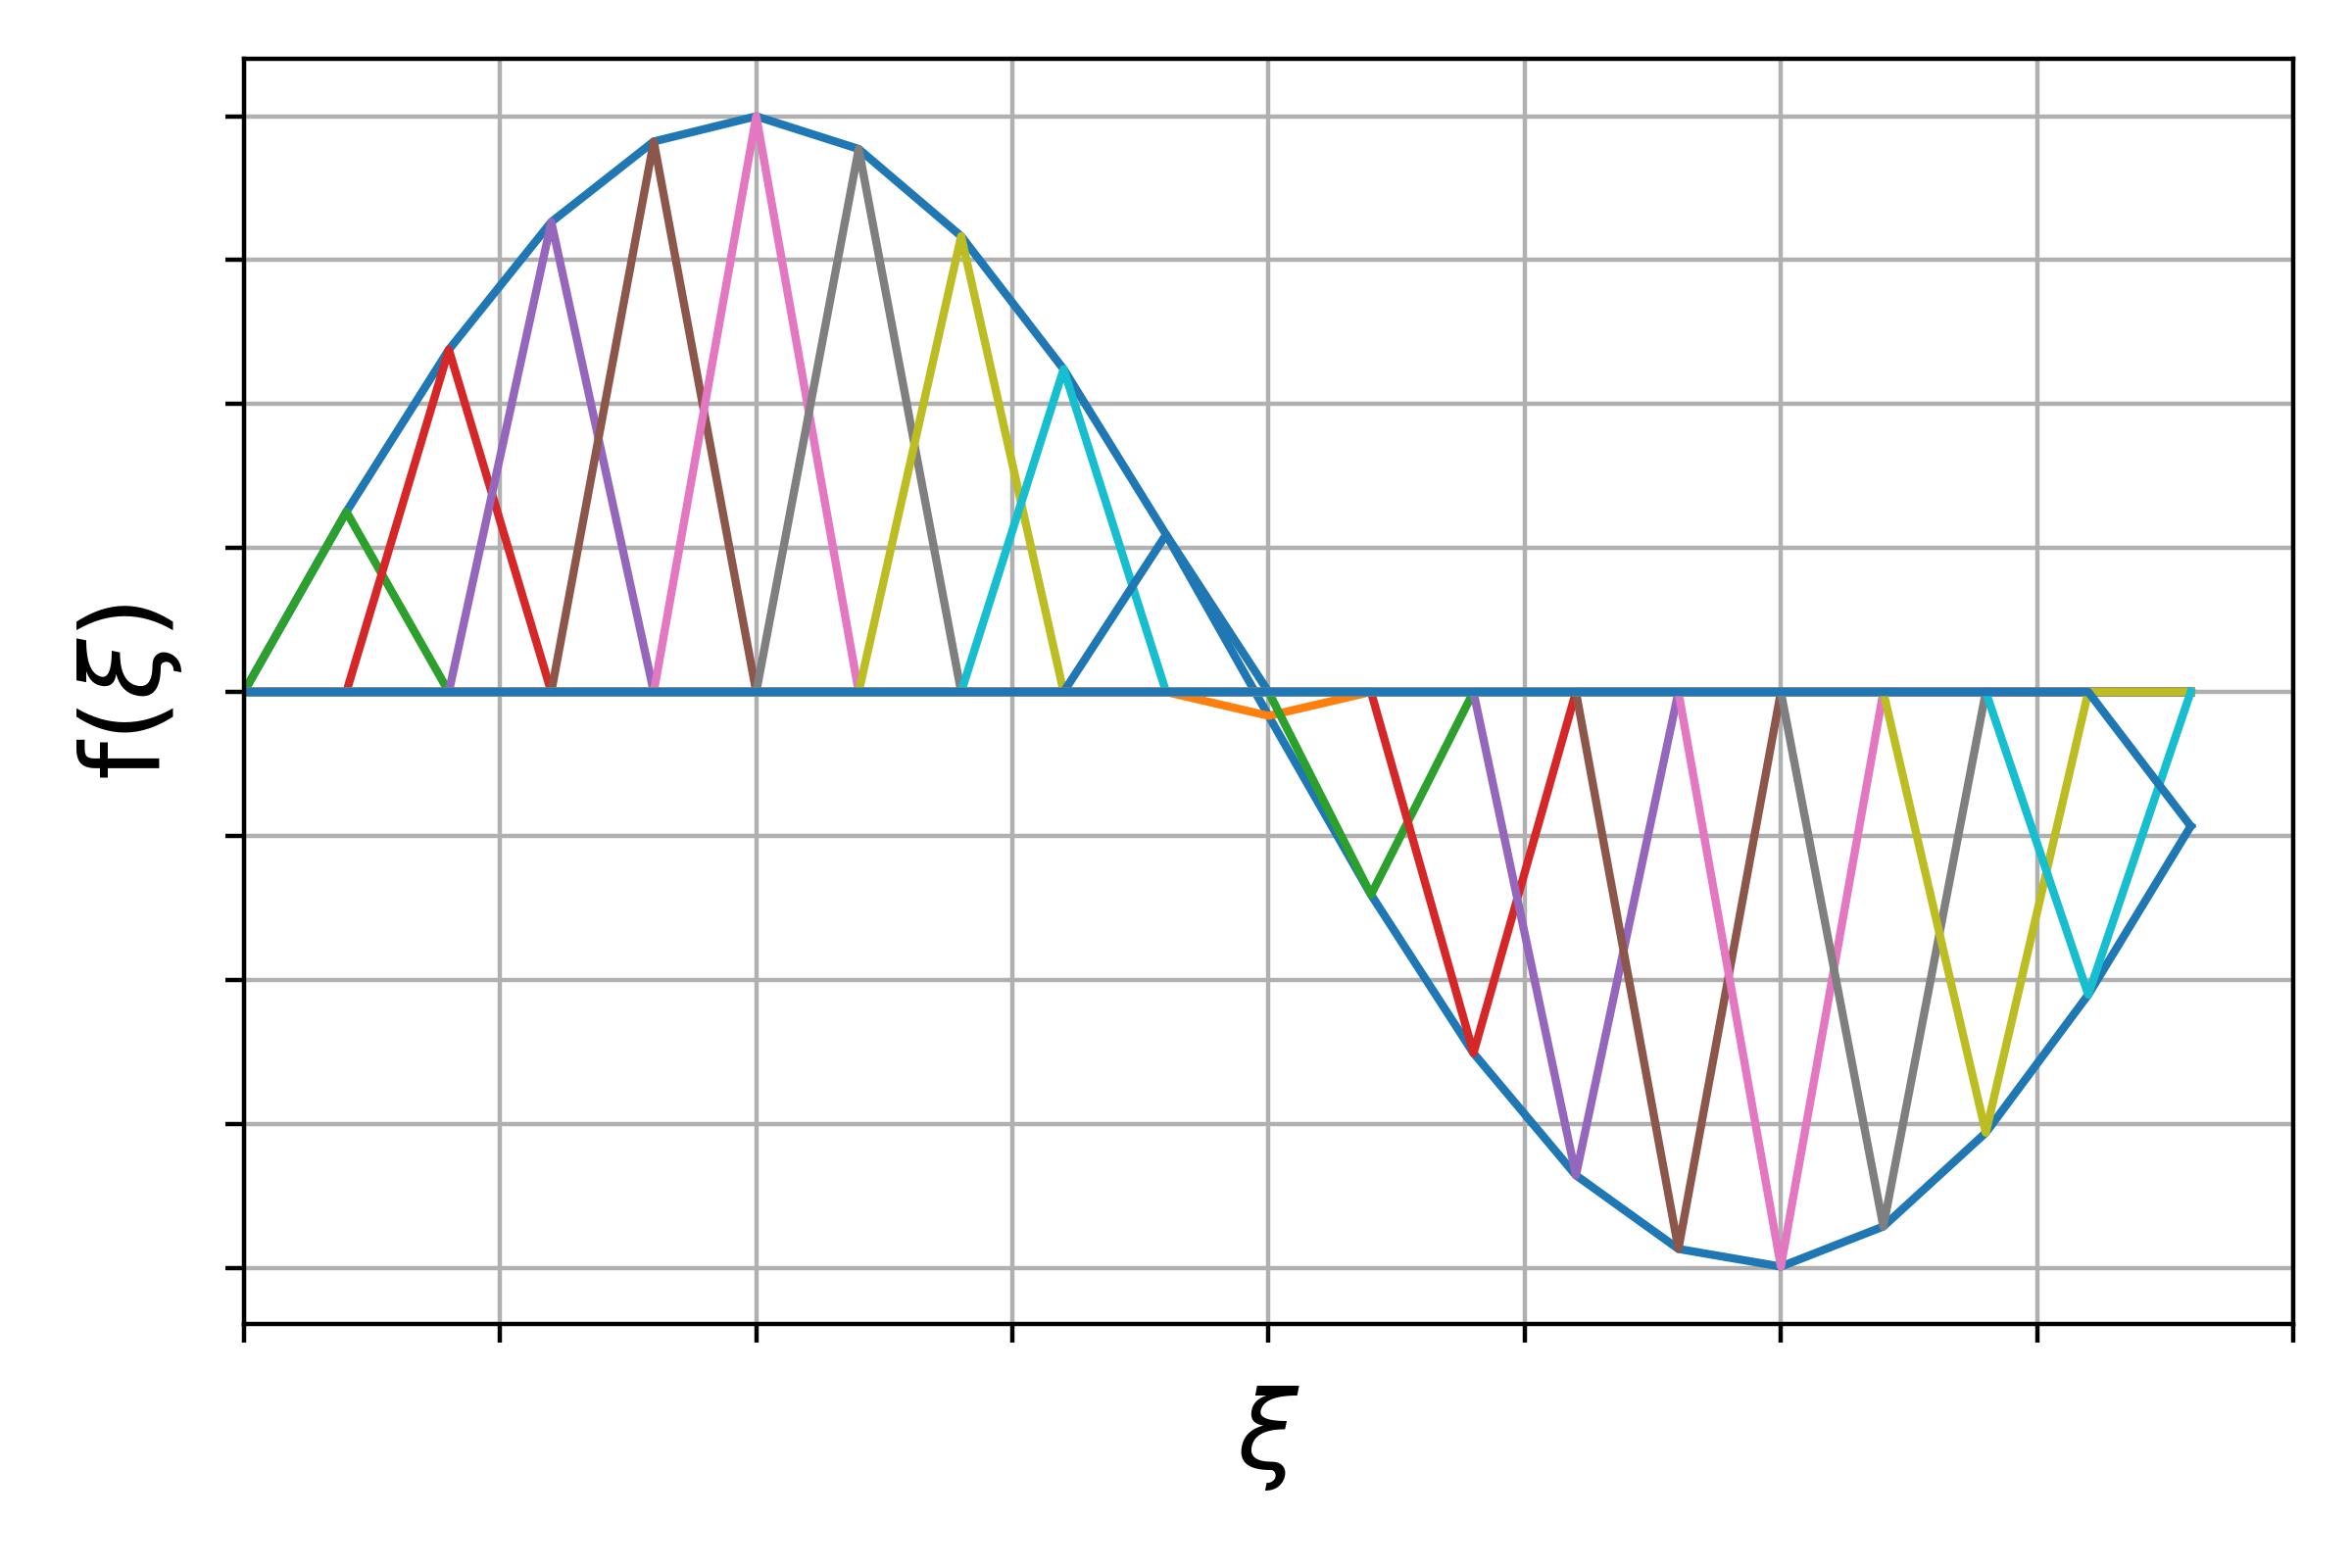
\includegraphics[width=0.45\textwidth]{bilder/FEM_1D} }}
    \subfloat[Illustration of numerical grid used for FEM integration of ABF-forces in 2D. Blue are original data points and orange control points obtained by linear interpolation. One 2D tent function is centered on each blue point.]{{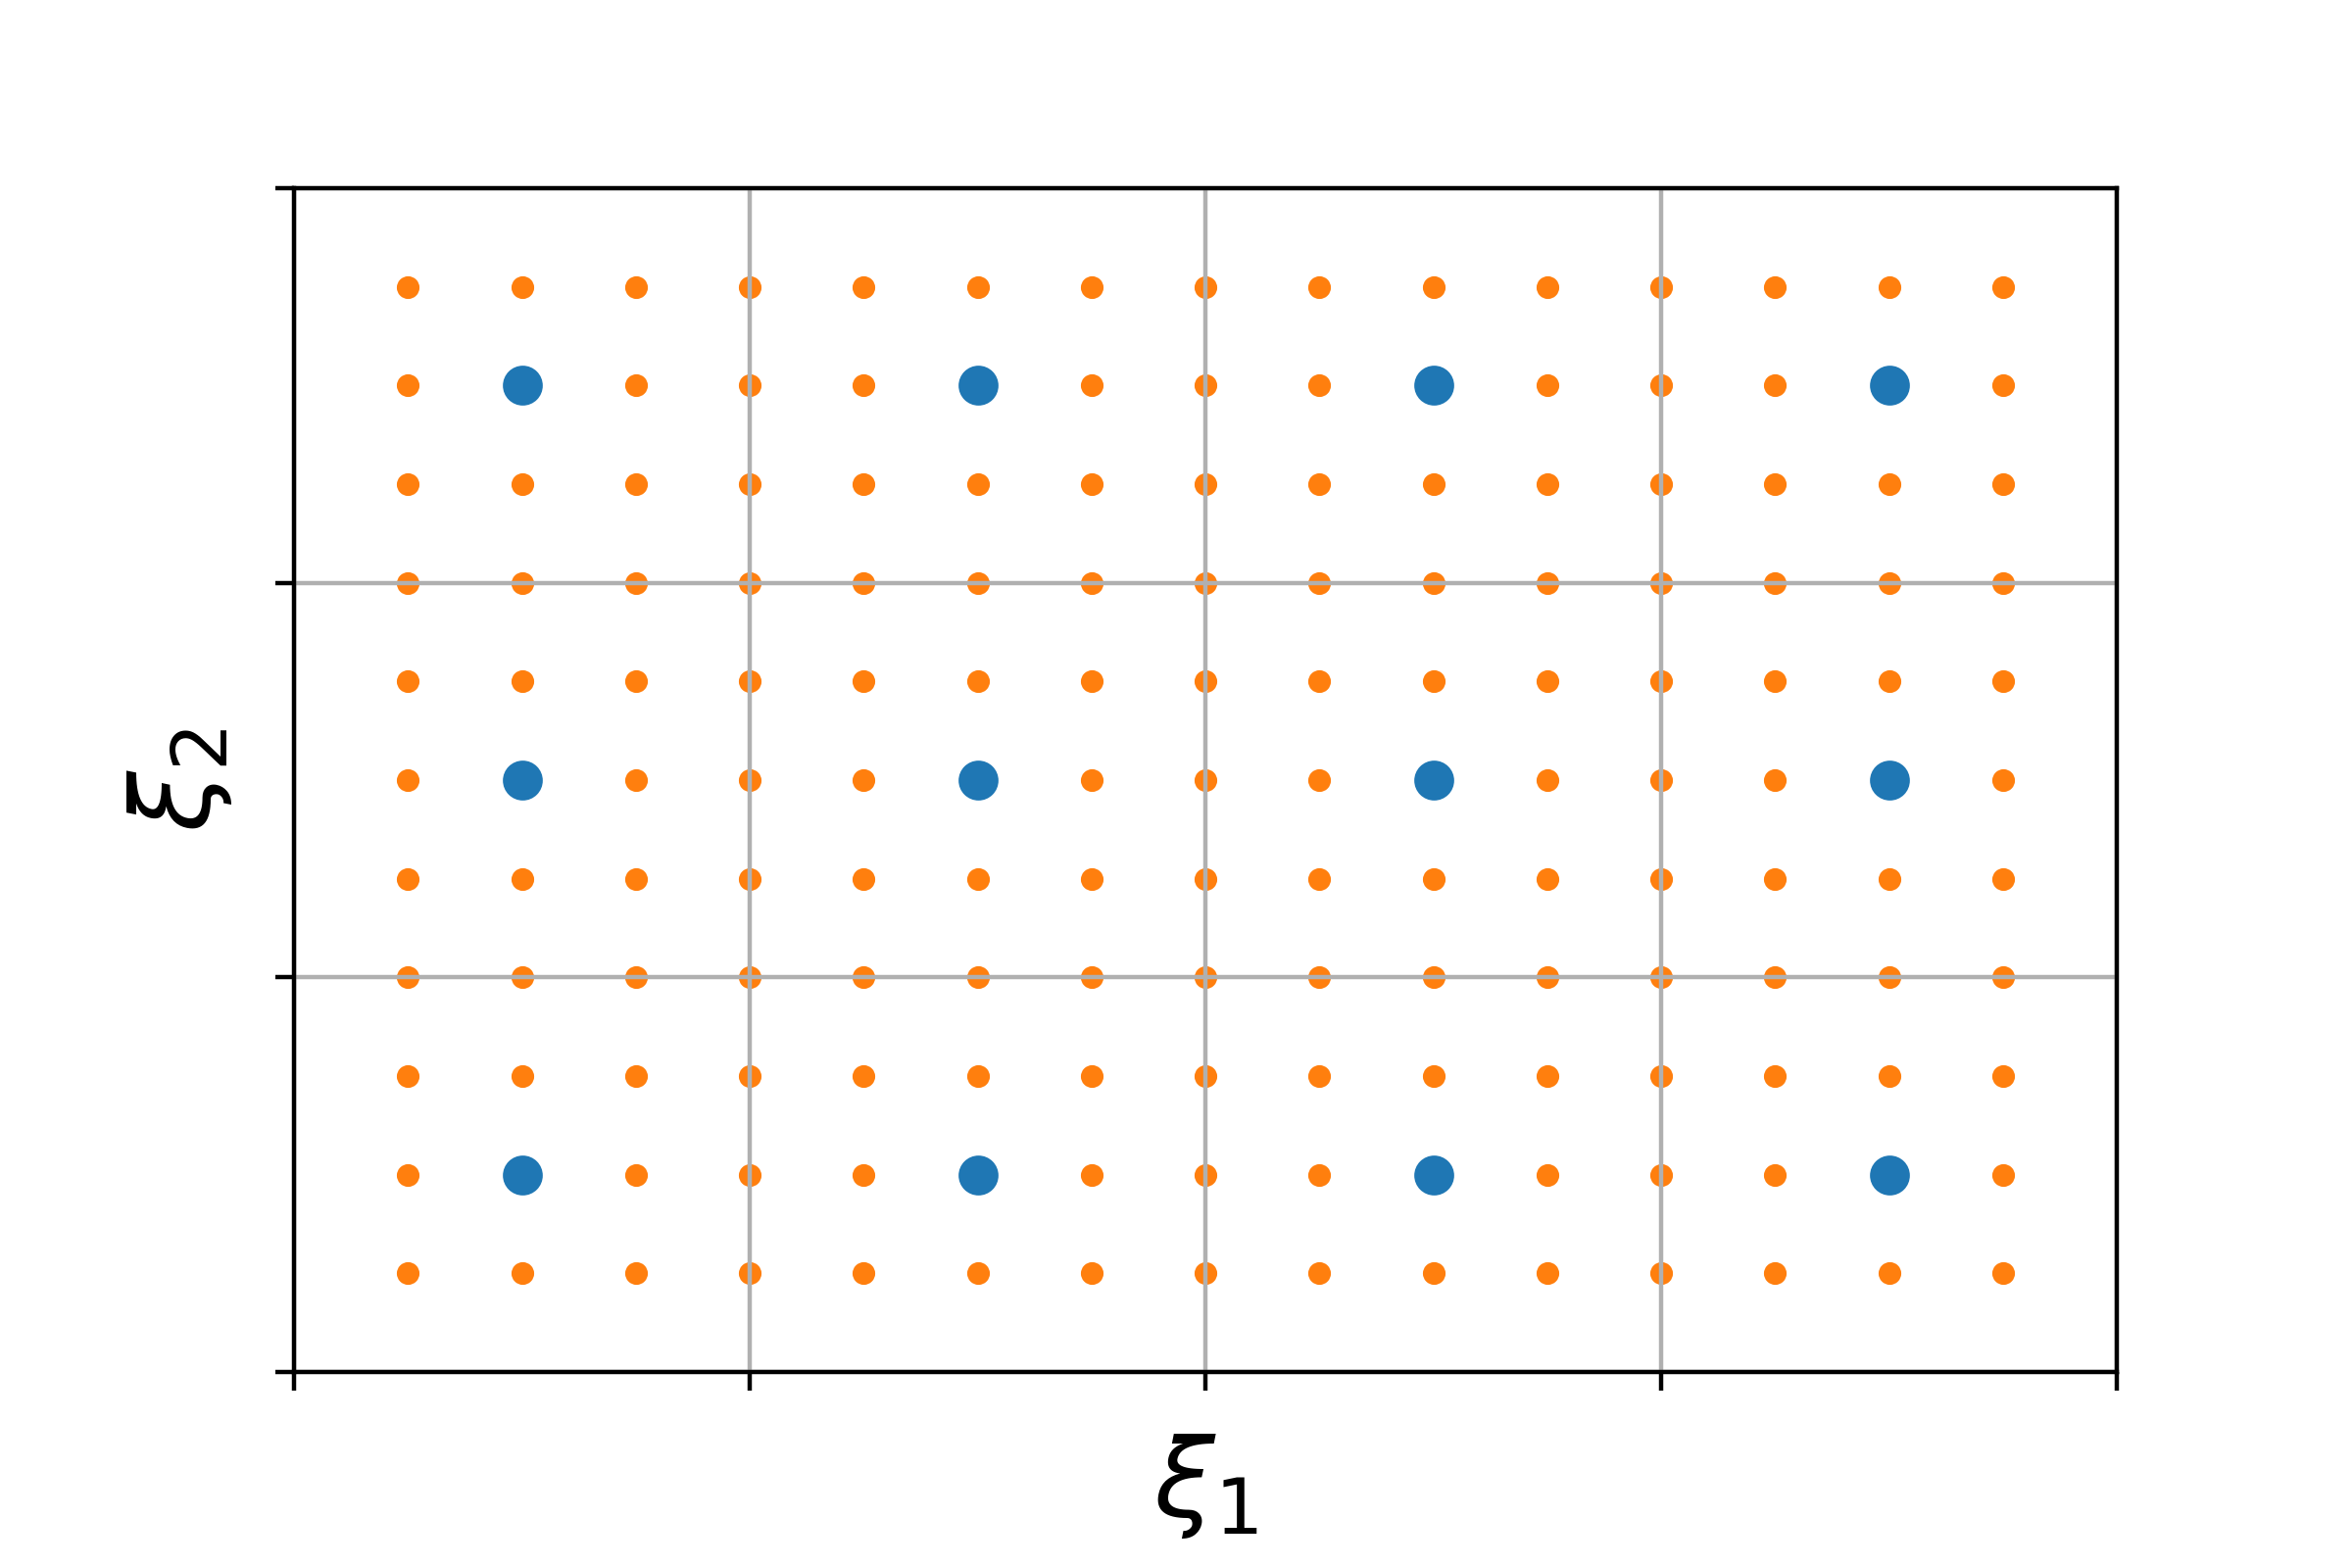
\includegraphics[width=0.5\textwidth]{bilder/grid} }}
\label{fig:FEM}%
\end{figure}


The last and critical ingredient for the ABF method now is an explicit expression for the instantaneous force $F_{\xi}$. Carter et al.\autocite{carter1989constrained} gave a first general expression:
\begin{equation}
  F(\xi,\textbf{q}) = -\frac{\partial V(\xi,\textbf{q})}{\partial \xi} + \beta^{-1} \frac{\partial \ln|J(\xi,\textbf{q})|}{\partial\xi} \label{eq:instforce old}
\end{equation}
which depends implicitly on a vector field $\partial x_i / \partial \xi$, hereafter referred to as "inverse gradient" and on an Jacobian correction term purely geometric in origin. The inverse gradient can be thought of as direction along which an infinitesimal change in $\xi$ is propagated in Cartesian coordinates, the complementary coordinates $\textbf{q}$ being kept constant. A major drawback of this formalism is the requirement of an full coordinate transform from Cartesian coordinates ($\textbf{x}$) to generalized coordinates ($\xi$, $\textbf{q}$).

This requirement could be lifted by den Otter\autocite{den2000thermodynamic}, who put forward the breakthrough idea that the change in $\xi$ can be propagated along an arbitrary vector field $\textbf{v}_i$ ($\mathbb{R}^{3N} \to \mathbb{R}^{3N}$), provided it satisfies some orthonormality conditions.
Extended to multidimensional reaction coordinates \textbf{$\xi$} = ($\xi_i$) and in presence of a set of constraints $\sigma_{k}(\textbf{x})=0$ these read:\autocite{ciccotti2005blue}
\begin{equation}
  \textbf{v}_i \cdot \nabla \xi_j = \delta_{ij} \label{eq:cond1}
\end{equation}
\begin{equation}
  \textbf{v}_i \cdot \nabla \sigma_k = 0 \label{eq:cond2}
\end{equation}
If all reaction coordinates $\xi_i$ are orthogonal to one another and to all constraints, $\textbf{v}_i = \nabla \xi_j/|\nabla \xi_j|^2$ is always a valid, but not necessarily the best, option.
Otherwise conditions \ref{eq:cond1} and \ref{eq:cond2} can be fulfilled by orthogonalization:\autocite{ciccotti2005blue}
\begin{equation}
  v_i (\textbf{x}) = \frac{Q^i \nabla \xi_i (\textbf{x})}{|Q^i \nabla \xi_i (\textbf{x})|} \label{eq:ortho v}
\end{equation}
with projector $Q^i$ given by the orthonormal basis $\{\hat{n}|_{j}^{i}(\textbf{x})\}_{j\neq i}$ in the subspace spanned by $\{\nabla \xi_j (\textbf{x})|\}_{j\neq i} \cup \{\nabla\sigma_j (\textbf{x})|\}_{j=1,...,M}$:
\begin{equation}
  Q^i = \textbf{1} - \sum_{j \neq i} \hat{n}_{j}^{i}(\textbf{x}) \otimes \hat{n}_{j}^{i}(\textbf{x})
\end{equation}
Replacing the inverse gradient by vectorfield $\textbf{v}_i$, expression \ref{eq:instforce old} finally reduces to:
\begin{equation}
  F(\xi_i,\textbf{x}) = -\nabla V(\textbf{x}) \cdot \textbf{v}_i(\textbf{x}) + \beta^{-1} \nabla \cdot \textbf{v}_i(\textbf{x})
\end{equation}
but still involves the calculation of second derivatives in the form of the divergence of vector fields $\textbf{v}_i$.\autocite{comer2015adaptive} Analytic expressions for bend angles and torsion angles, used in the present work, are given in the appendix. However, especially for torsion angles orthogonalization via equation \ref{eq:ortho v} becomes exceedingly tedious and inpracticel, significantly limiting the applicability of ABF for multidimensional reaction coordinates.

%\subsection{extended Adaptive Biasing Force Method (eABF)}
%\label{sec:eABF}
To circumvent the technical requirements of ABF Lesage et al.\autocite{lesage2017smoothed} proposed an more flexible approach named eABF.
In eABF the physical system is extended by additional coordinates $\lambda$ with mass $m_{\lambda}$, which are coupled to the reaction coordinates $\xi_i$ with harmonic potentials. The extended system ($\textbf{x}$, $\lambda$) evolves according to Langevin dynamics in the extended potential
\begin{equation}
  V^{ext}(\textbf{x},\lambda_i) = V(\textbf{x}) + \frac{k_i}{2}(\xi_{i}(\textbf{x})-\lambda_i)^2.
\end{equation}
The key intuition behind eABF is, that in the tight coupling limit efficient sampling of $\lambda$ will result in efficient sampling of $\xi$. Therefore, to obtain uniform sampling along $\xi$ biasing of $\lambda$ is sufficient. The inverse gradient is chosen as null for all physical coordinates $\textbf{x}$ and 1 for $\lambda$. This way constraints \ref{eq:cond1} and \ref{eq:cond2} are always satisfied, which is especially useful for calculations involving a set of non-orthogonal reaction coordinates.
Sampling the extended system gives the following unbiased Boltzmann distribution in $\lambda$:
\begin{equation}
\begin{aligned}
  \rho^k(\lambda) &\propto
  \int \exp \biggl[-\beta \biggl(V(\textbf{x})+\frac{k}{2}(\xi(\textbf{x})-\lambda)^2 \biggr) \biggr] d\textbf{x} \\
  &= \int \exp \biggl[-\beta V(\textbf{x}) - \frac{(\xi(\textbf{x})-\lambda)^2}{2\sigma^2} \biggr] d\textbf{x}
\end{aligned}
\end{equation}
which depends on the force constant $k$ or variance of the Gaussian kernel $\sigma^2=(\beta k)^{-1}$.
The bias on $\lambda$ is the running average over the spring force in $\lambda$-bin k:
\begin{equation}
  \overline{F}(\lambda_{i}, k) = \frac{\partial A^{k}(\lambda_{i})}{\partial \lambda_i} = \frac{1}{N_{Step}^{k}} \sum_{\mu=1}^{N_{Step}^{k}} k(\lambda_{i,\mu}^{k}-\xi_{i,\mu}^{k})
\end{equation}
For small values of $N_{Step}^{k}$ again the linear ramp function $R(N_{Step},k)$ given by equation \ref{eq:ramp} is used. This generates the following biased Boltzmann distribution:
\begin{equation}
  \tilde{\rho}(\lambda) \propto \int \exp \biggl[-\beta V(\textbf{x})-\frac{(\xi(\textbf{x})-\lambda)^2}{2\sigma^2} + A^{k}(\lambda) \biggr) \biggr] d\textbf{x}
\end{equation}
By using $\int \delta(\xi(\textbf{x})-z)dz=1$ and $A^k(\lambda)=-\beta^{-1}\ln\rho^k(\lambda)$ one can obtain the relationship between unbiased and biased z-distributions:
\begin{equation}
  \tilde{\rho}(z) =  \rho(z) \int \frac{\exp \bigl(-\frac{(\lambda-z)^2}{2\sigma^2}\bigr)}
  {\int \exp\bigl(-\frac{(\lambda-z')^2}{2\sigma^2}\bigr)\rho(z')dz'} d\lambda
\end{equation}
For the tight coupling limit (high $k$, low $\sigma$) the unbiased distribution $\rho(z)$ is recovered and eABF recovers the behavior of standard ABF.
In this case $A^k(\lambda)$  approximates the physical free energy $A(z)$ and the $\Delta A_{z}$ can be approximated by integrating over the converged bias forces on $\lambda$, $\overline{F}(\lambda_{i}, k)$, which will be referred to as "naive estimator" (eABF/naive) hereafter.

An asymptotically unbiased estimator of the free energy can be derived by correcting the free energy gradient obtained from the eABF-biased distribution $\tilde{\rho}(z)$ with the average biasing force on z
\begin{equation}
  \frac{\partial A(z)}{\partial z_i} = -\beta^{-1}\frac{\partial \ln \tilde{\rho}(z)}{\partial z_i} + k(\braket{\lambda_i}_{z}-z_{i})
\end{equation}
which is called "Corrected z-averaged restraint" (CZAR) and can be calculated numerically from the time trajectory ($z_i$,$\lambda_i$) in an post-processing step.\autocite{lesage2017smoothed}

\subsection{Meta-eABF}
\label{sec:meta-eABF}

\section{Standard vs geometric free energy}
